\subsection{State Estimation}
\subsubsection{Overview}
The first question is whether the pipeline can produce a state estimate that is good enough for stable sonar map generation. Local maps are only as good as the poses used to place each sonar swath, so trajectory drift, sensor dropouts, and inconsistent orientation estimates directly reduce map quality and later landmark accuracy. The state estimator is therefore evaluated to determine whether it provides physically reasonable motion estimates under realistic underwater conditions.
\\ \\
The state estimation component was evaluated using the recorded LAUV dataset described in the previous section. The estimator implemented in this work is based on the Unscented Kalman Filter on Manifolds (UKF-M), which allows the filter to operate directly on nonlinear state spaces such as $SO(3)$ for orientation. This avoids manually maintaining rotation Jacobians and provides a practical framework for inertial navigation and sensor fusion.
\\ \\
For reference, the results are compared against the navigation solution generated by the onboard LAUV navigation stack. The onboard system uses a model based Extended Kalman Filter (EKF) with a predefined kinetic vehicle model and operational constraints. This solution is not treated as ground truth, but is used as a benchmark to verify that the implemented estimator produces physically consistent and comparable behaviour.
\\ \\
The estimator developed in this thesis uses a purely inertial kinematic model combined with external aiding sensors such as DVL, depth, GNSS, and AHRS measurements. Without a predefined hydrodynamic vehicle model, the estimator depends more directly on the available sensor measurements. When aiding sensors become unavailable, the estimator must rely on inertial dead reckoning, which naturally introduces drift over time.
\\ \\
The dataset contains several periods where aiding sensors are unavailable. GNSS measurements are lost when the vehicle operates underwater, and DVL measurements may drop out depending on altitude and seabed conditions. These conditions make the dataset useful for evaluating estimator robustness and for showing why SLAM is needed. Inertial navigation can support short term motion estimation, but long term consistency requires environmental constraints such as sonar landmarks and loop closures.



\subsubsection{Parameters}
The main filter parameters used in the experiments are summarized in Table \ref{tab:ukf_params}. These parameters define the assumed uncertainty in the initial state, process model, and sensor measurements.
\begin{table}[H]
    \centering
    \caption{State estimator parameters}
    \label{tab:ukf_params}
    \begin{tabular}{l l}
        \hline
        Parameter & Value \\
        \hline
        Initial position std & 10 m \\
        Initial velocity std & 1.0 m/s \\
        Initial orientation std & 0.1 rad \\
        Depth sensor std & 0.05 m \\
        DVL velocity std & 0.002 m/s \\
        Accelerometer std & 2.0 m/s$^2$ \\
        Gyroscope std & 0.05 rad/s \\
        AHRS orientation std & 0.01 rad \\
        Sigma point spread parameter $\alpha$ & $10^{-3}$ \\
        \hline
    \end{tabular}
\end{table}
\noindent
The accelerometer process noise was intentionally set higher than typical IMU specifications. This tuning choice compensates for unmodeled environmental effects such as hydrodynamic forces, currents, and vehicle dynamics that are not explicitly represented in the purely kinematic motion model used by the filter.



\newpage



\subsubsection{Benchmark Comparison}
Figures \ref{fig:results-state-estimation-position}--\ref{fig:results-state-estimation-orientation} compare the estimated states with the reference navigation solution recorded during the mission.
\begin{figure}[H]
    \centering
    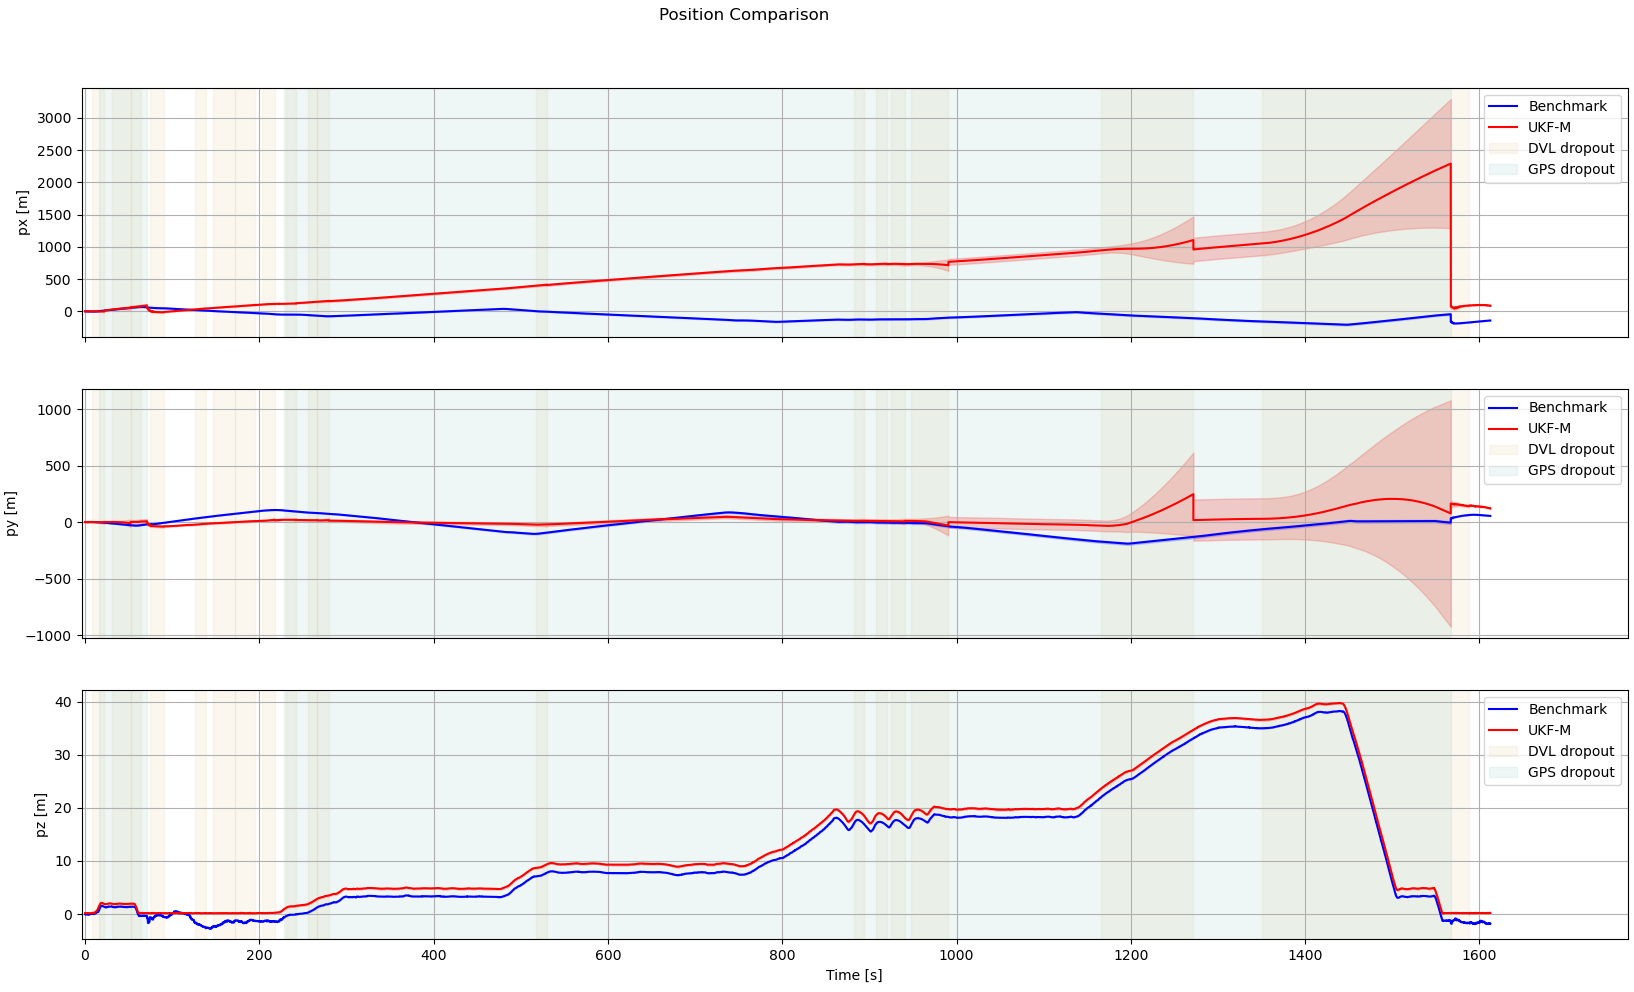
\includegraphics[width=0.7\linewidth]{Pictures/Results/State_Estimation/Benchmark_Position_zoom_out.png}
    \caption{Comparison of estimated and reference vehicle position. Vertical position remains accurate due to reliable depth measurements, while horizontal drift increases during periods of sensor dropout.}
    \label{fig:results-state-estimation-position}
\end{figure}
\noindent
The depth estimate closely follows the reference trajectory, which is expected since the pressure sensor provides reliable and continuous measurements. In contrast, horizontal position estimates gradually diverge during periods where GNSS and DVL measurements are unavailable. During these intervals the estimator relies solely on inertial propagation, resulting in accumulated drift.
\begin{figure}[H]
    \centering
    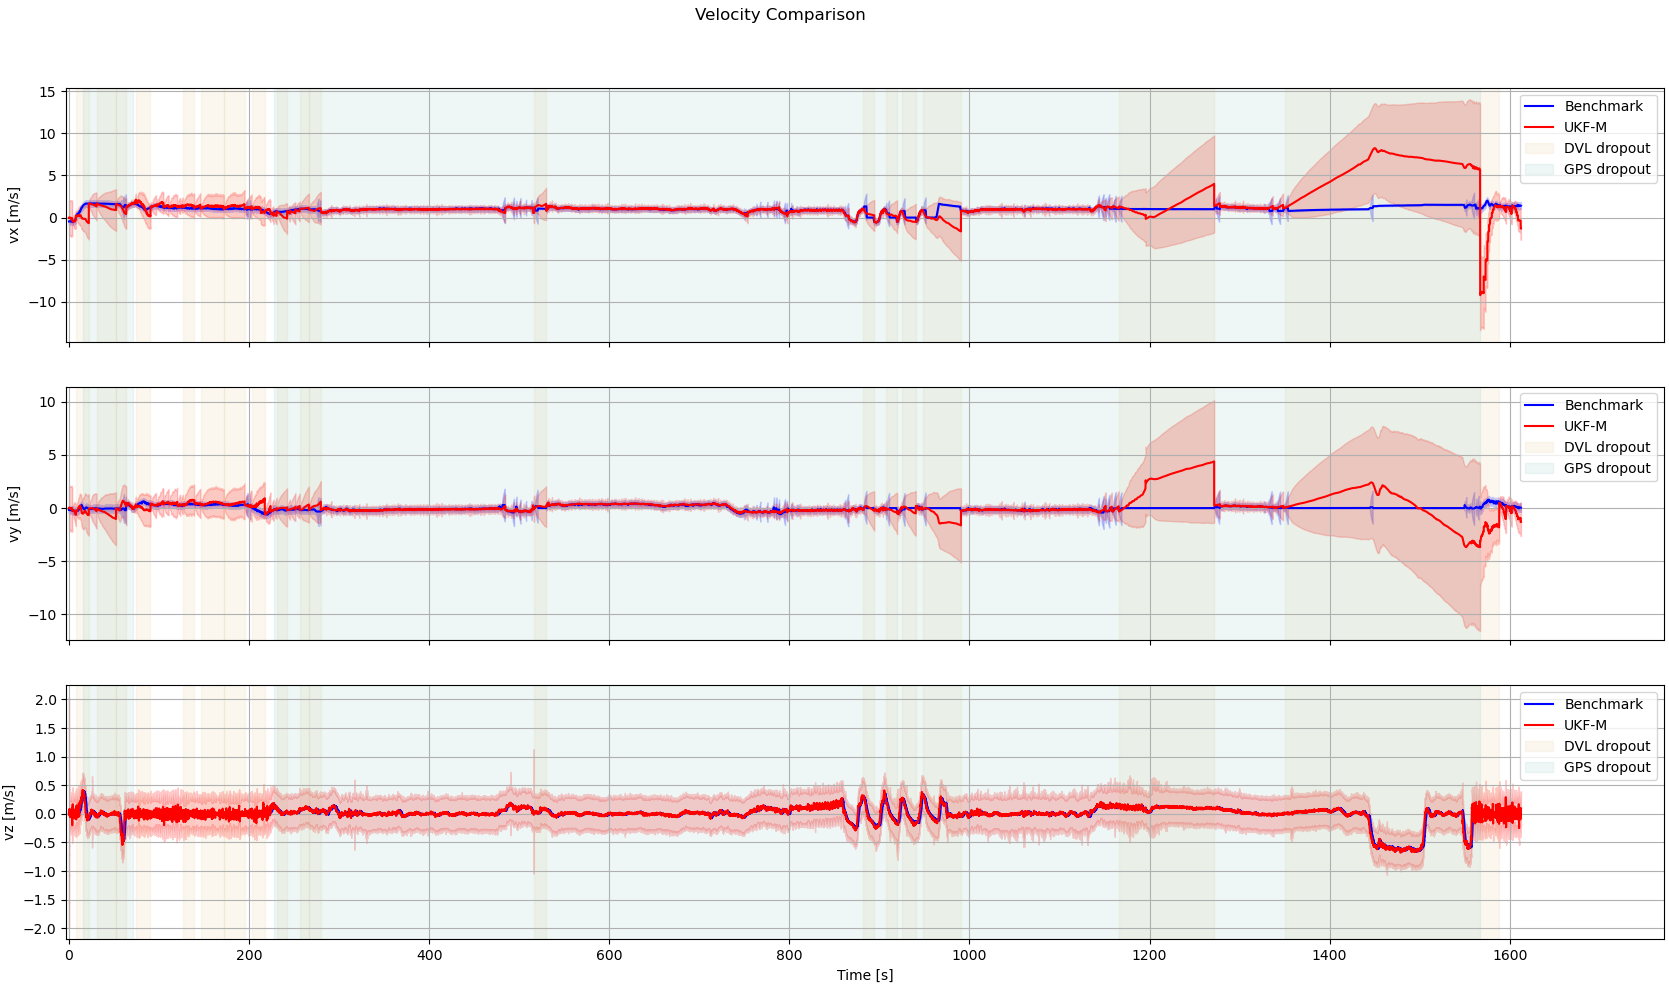
\includegraphics[width=1.0\linewidth]{Pictures/Results/State_Estimation/Benchmark_Velocity_zoom_out.png}
    \caption{Comparison of estimated and reference vehicle velocity. Good agreement is observed when DVL measurements are available.}
    \label{fig:results-state-estimation-velocity}
\end{figure}
\noindent
Velocity estimates remain consistent with the reference solution for most of the trajectory. This indicates that the inertial propagation combined with DVL aiding provides reliable velocity estimates when measurements are available.

\newpage

\begin{figure}[H]
    \centering
    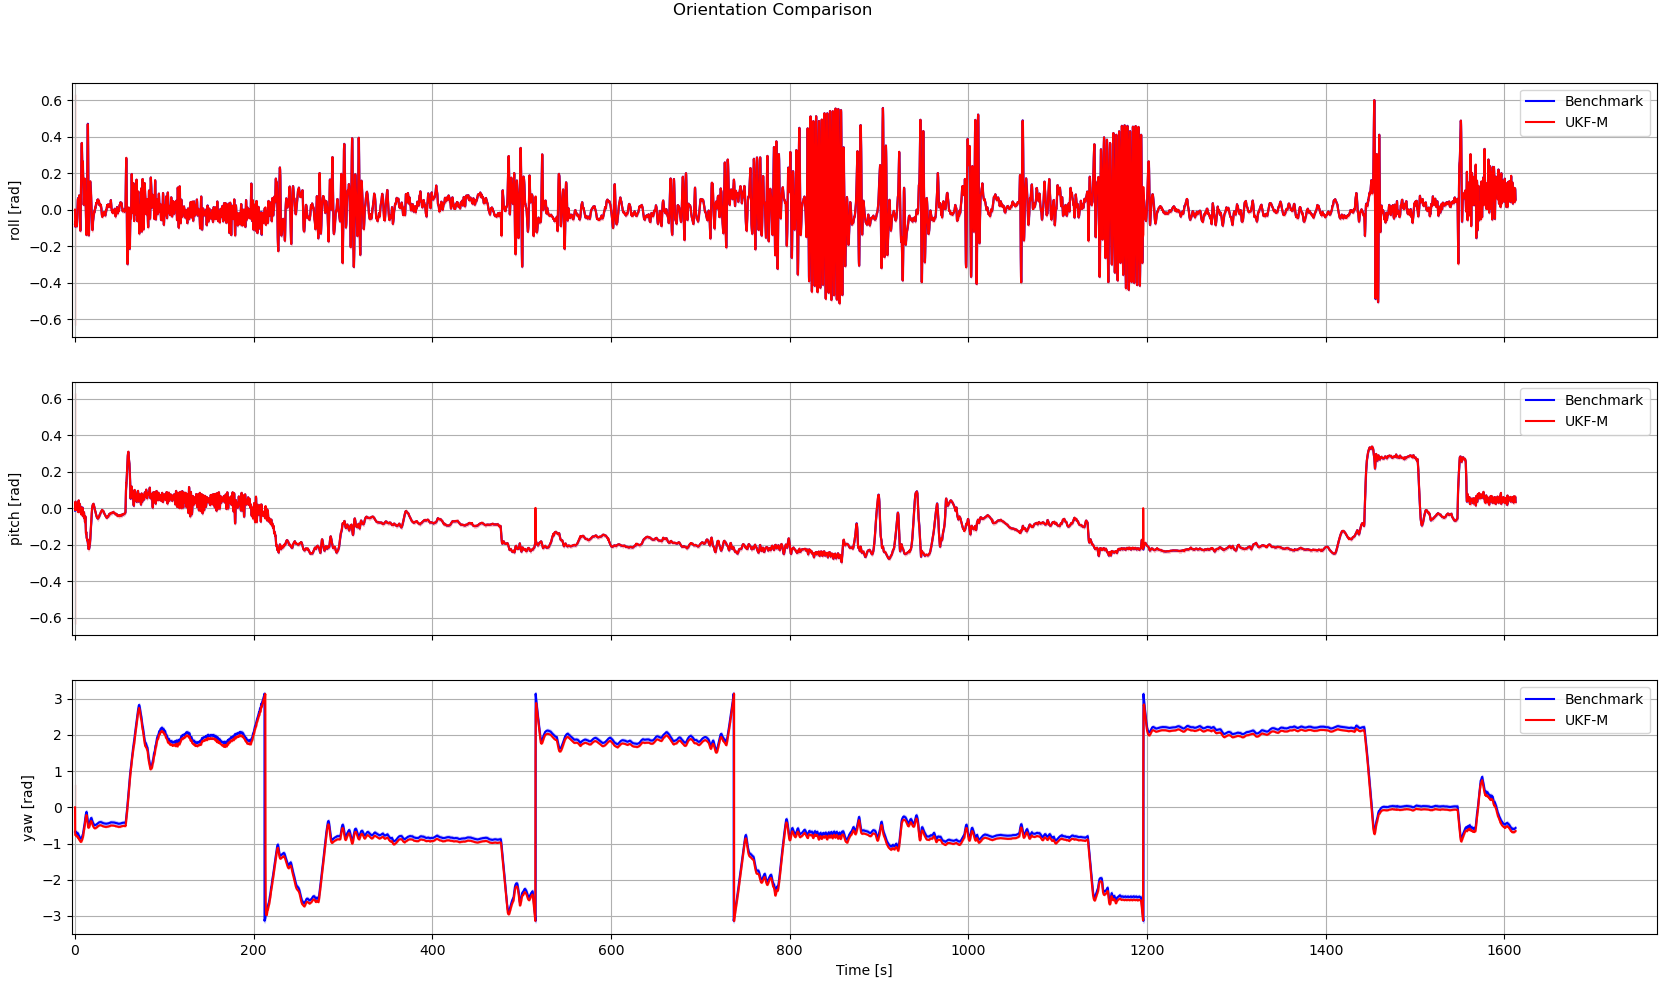
\includegraphics[width=1.0\linewidth]{Pictures/Results/State_Estimation/Benchmark_Orientation_zoom_out.png}
    \caption{Comparison of estimated and reference vehicle orientation. The estimator accurately tracks the reference orientation throughout the trajectory.}
    \label{fig:results-state-estimation-orientation}
\end{figure}
\noindent
The orientation estimates show strong agreement with the reference solution throughout the mission. This behavior is expected because the AHRS provides stable attitude measurements that strongly constrain the rotational states.



\newpage



\subsubsection{NIS Consistency Tests}
Normalized Innovation Squared (NIS) tests were performed to evaluate filter consistency for the different sensor measurements. The NIS metric compares the innovation statistics with the predicted covariance of the filter.
\begin{figure}[H]
    \centering
    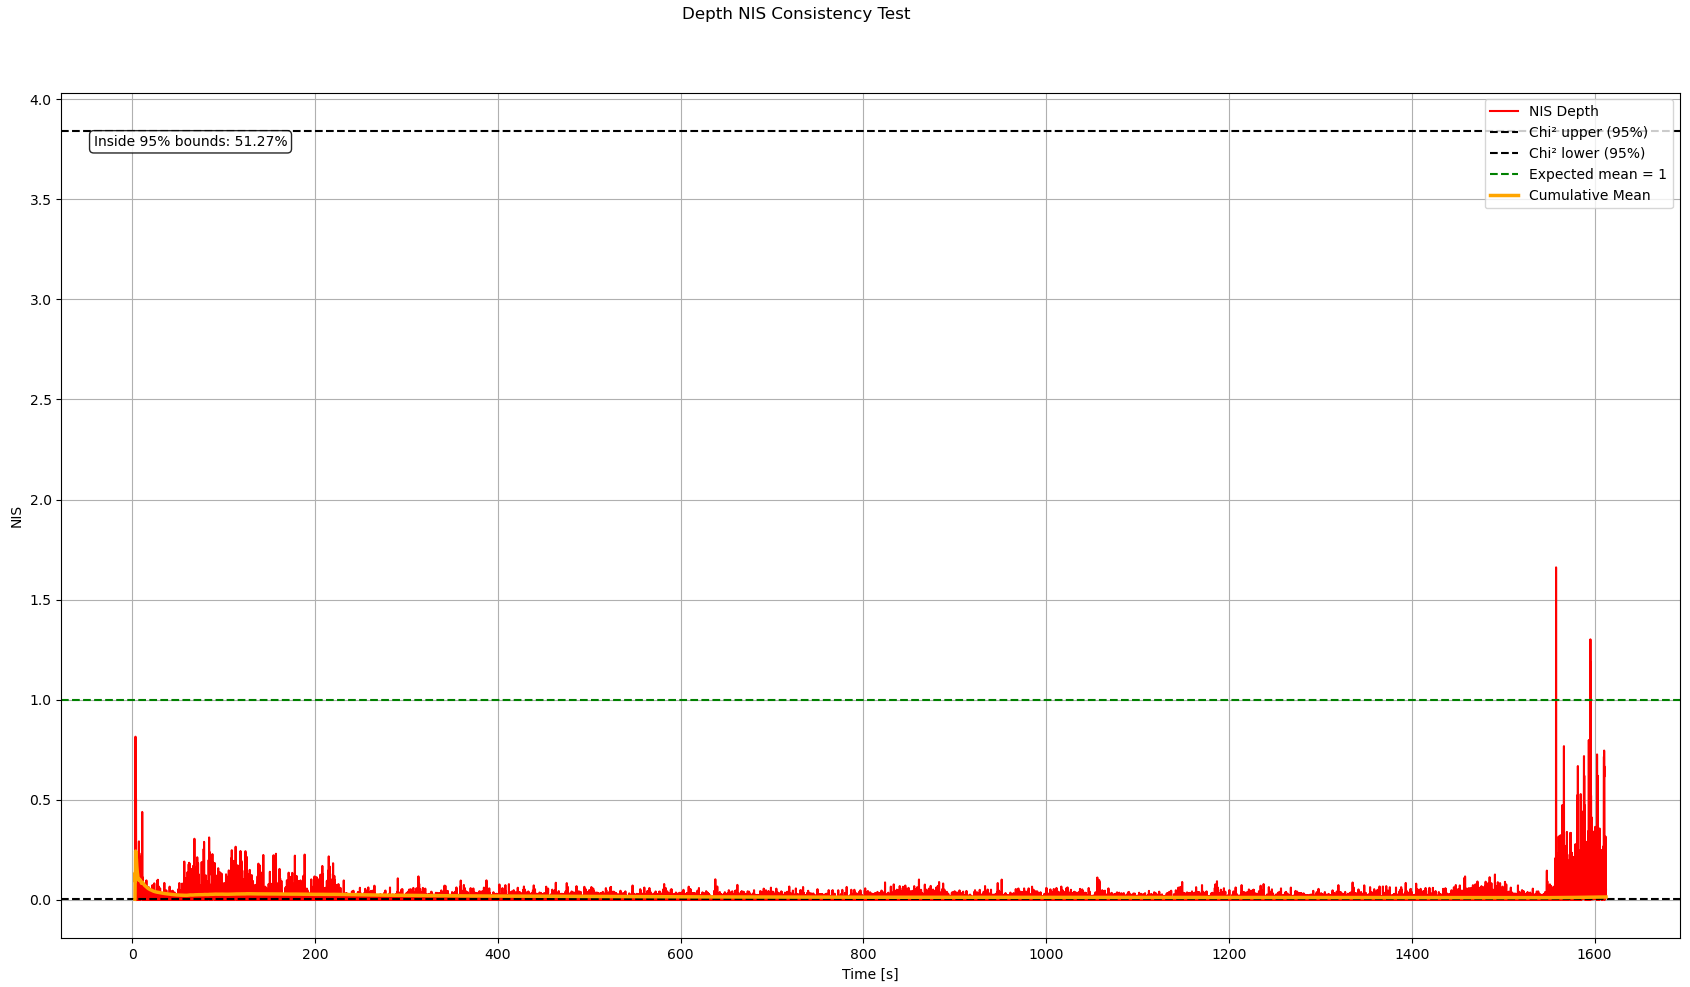
\includegraphics[width=0.7\linewidth]{Pictures/Results/State_Estimation/NIS_Depth_zoom_out.png}
    \caption{NIS consistency test for the depth sensor. Most innovations remain within the expected confidence bounds.}
    \label{fig:results-state-estimation-nis-depth}
\end{figure}
\noindent
The depth sensor shows stable and consistent behavior with most innovations remaining within the expected statistical bounds. This indicates that the measurement noise model for the depth sensor is well tuned.
\begin{figure}[H]
    \centering
    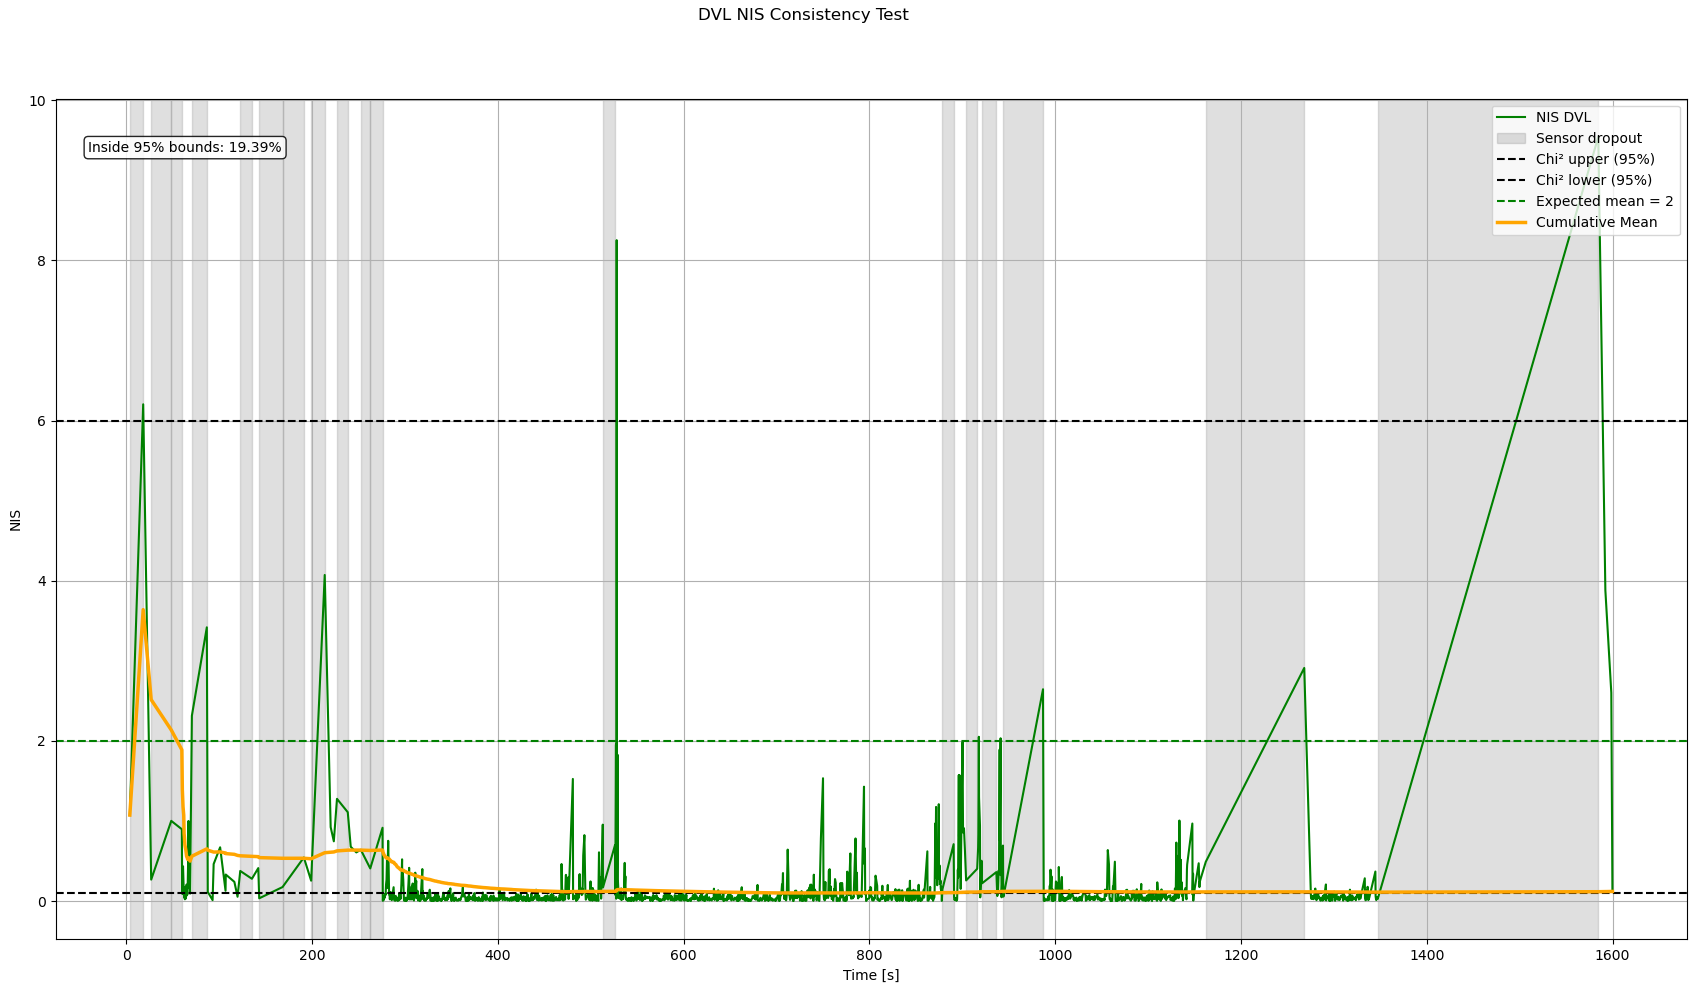
\includegraphics[width=1.0\linewidth]{Pictures/Results/State_Estimation/NIS_DVL_zoom_out.png}
    \caption{NIS consistency test for the DVL velocity measurements. Measurement dropouts lead to increased prediction uncertainty.}
    \label{fig:results-state-estimation-nis-dvl}
\end{figure}
\noindent
For the DVL measurements, the NIS values remain low during normal operation but increase when measurements become unavailable. These intervals correspond to periods where the estimator must rely on inertial propagation, which increases uncertainty until aiding measurements return.

\newpage

\begin{figure}[H]
    \centering
    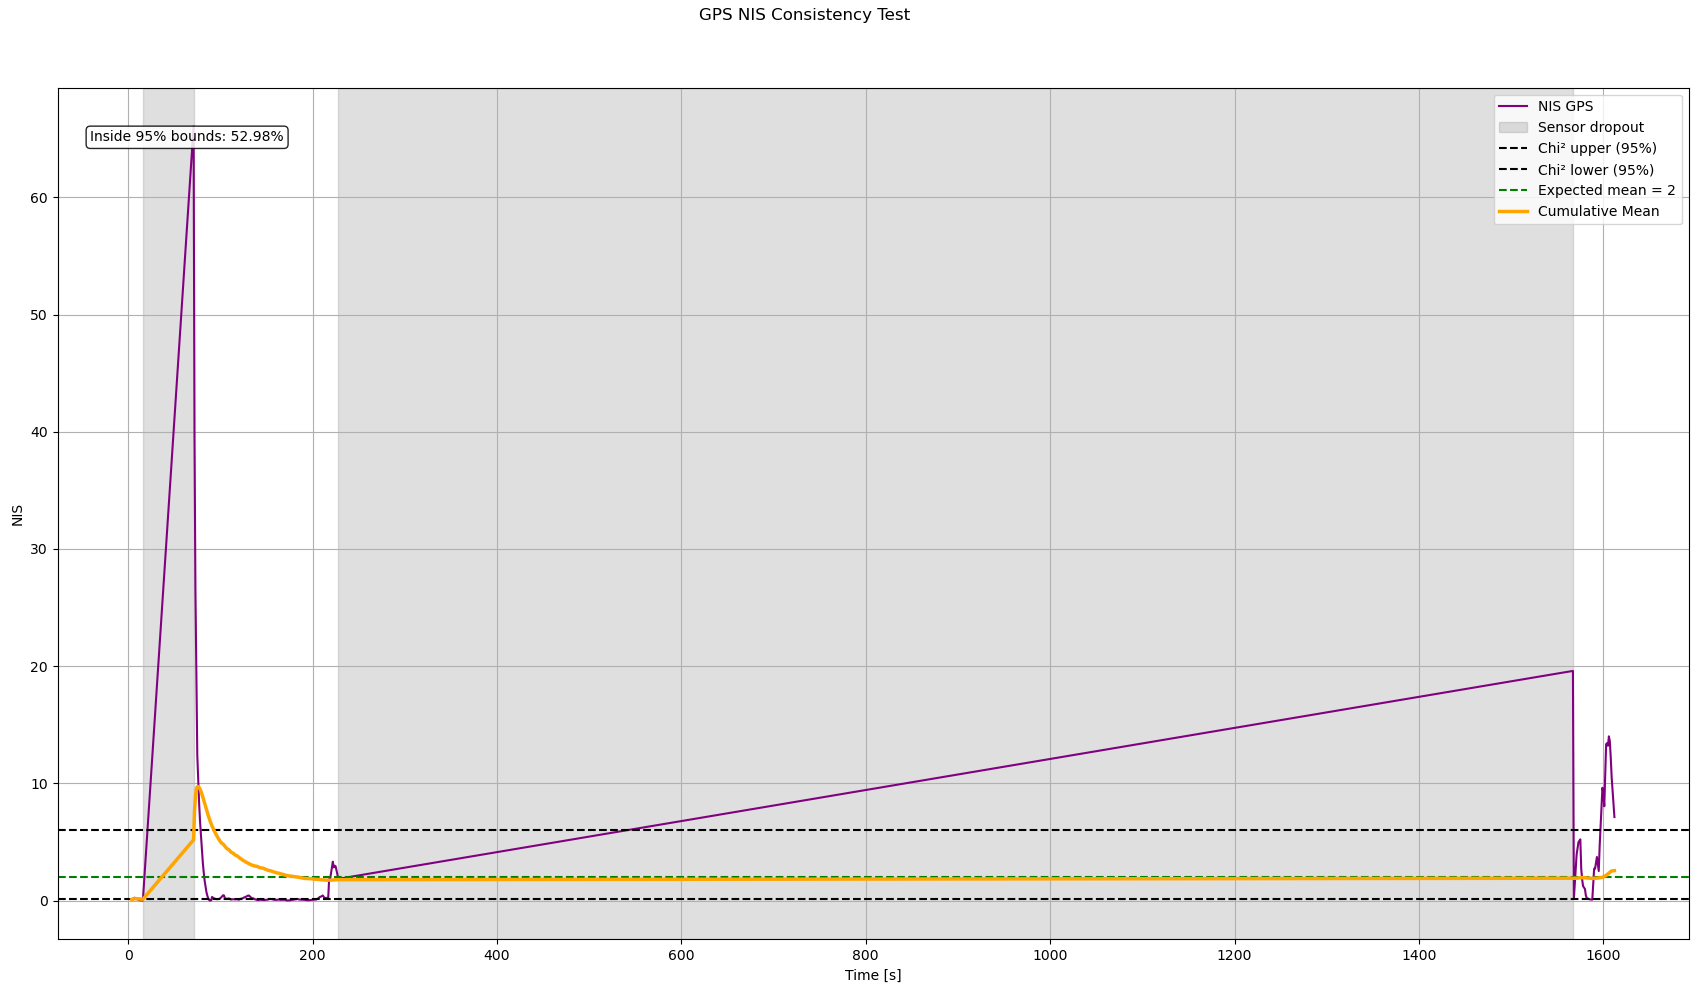
\includegraphics[width=1.0\linewidth]{Pictures/Results/State_Estimation/NIS_GPS_zoom_out.png}
    \caption{NIS consistency test for GNSS measurements. Large innovations occur when GNSS measurements return after extended underwater operation.}
    \label{fig:results-state-estimation-nis-gps}
\end{figure}
\noindent
GNSS measurements exhibit the largest innovations, which is expected due to extended periods where the vehicle operates underwater and GNSS is unavailable. When the vehicle resurfaces and GNSS measurements become available again, large corrections occur due to accumulated dead reckoning drift.
\\ \\
Overall, the NIS analysis suggests that the filter tends to be slightly conservative. This conservative tuning was intentionally chosen to ensure stable behavior during extended sensor dropout periods.



\newpage



\subsubsection{Performance}
\begin{figure}[H]
    \centering
    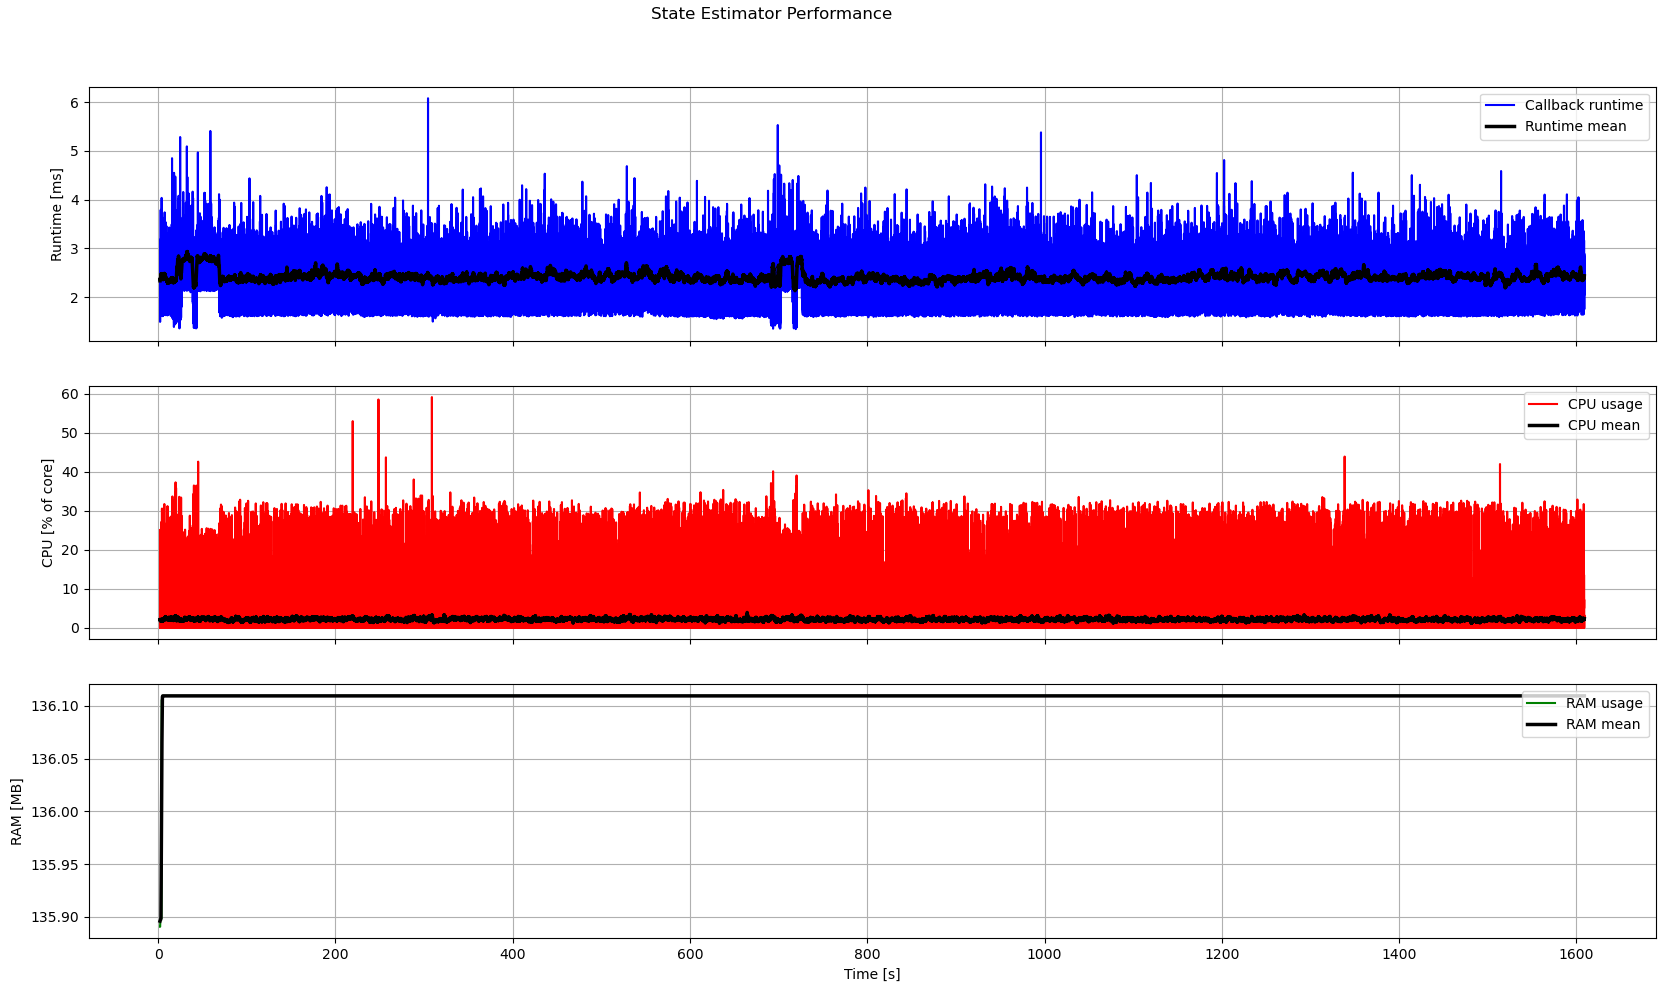
\includegraphics[width=1.0\linewidth]{Pictures/Results/State_Estimation/Performance.png}
    \caption{Runtime, CPU usage, and memory consumption of the state estimator during operation.}
    \label{fig:results-state-estimation-performance}
\end{figure}
\noindent
The computational performance of the estimator was evaluated by measuring runtime, CPU usage, and memory consumption during execution. The average callback runtime remains within a few milliseconds, which is sufficient for real time operation.
\\ \\
Despite using an Unscented Kalman Filter formulation and being implemented in Python, the estimator requires only minimal CPU resources. Most of the observed memory usage originates from the ROS2 middleware environment rather than the estimator itself. The algorithmic component of the estimator requires only a few megabytes of memory, while the total process footprint is dominated by ROS2 infrastructure.
\\ \\
These results demonstrate that the estimator is computationally lightweight and suitable for integration into the complete SLAM pipeline.
